\documentclass[a4paper,12pt]{article} % тип документа
\usepackage[margin=1in]{geometry} % Поля

%  Русский язык
\usepackage[warn]{mathtext}
\usepackage[T2A]{fontenc}			% кодировка
\usepackage[utf8]{inputenc}			% кодировка исходного текста
\usepackage[english,russian]{babel}	% локализация и переносы
% Математика
\usepackage{amsmath,amsfonts,amssymb,amsthm,mathtools} 
\usepackage{wasysym}
%%%
\usepackage{graphicx}

\usepackage{gensymb} % знак градуса
\usepackage{enumitem} % изменить список enumerate
\usepackage{placeins} % \FloatBarrier

%%%% Римские цифры
\renewcommand{\thesection}{\Roman{section}.} 
\renewcommand{\thesubsection}{\roman{subsection}.}

\begin{document}
%титул
\hrule 	
\medskip
\begin{raggedright}
{\large \textbf{Лабораторная работа 1.3.3}}
\\
\medskip
{\Large Измерение вязкости воздуха по течению в тонких трубках} 
\\
\medskip
{\large Карташов Констанин Б04-005}
\medskip
\hrule
\medskip
\end{raggedright}


\section{Анотация}

\paragraph{Цель работы:} 
\begin{enumerate}
\itemsep0em
\item Экспериментально исследовать свойства течения газов по тонким трубкам при различных числах Рейнольдса 
\item Выявить область применимости закона Пуазейля и с его помощью определить коэффициентвязкости воздуха
\end{enumerate}
\paragraph{Оборудование:}
\begin{itemize}
\renewcommand{\labelitemi}{$\triangleright$}
\itemsep0em
\item Система подачи воздуха (компрессор, поводящие трубки)
\item Газовый счётчик барабанного типа 
\item Спиртовой микроманометр с регулируемым наклоном 
\item Набор трубок различного диаметра с выходами для подсоединения микроманометра
\item Секундомер
\end{itemize}

\medskip\hrule\medskip

\section{Теоретическая часть}

\medskip\hrule\medskip

\section{Экспериментальная часть}

\subsection{Описание экспериментальной установки}

\begin{figure}
\centering
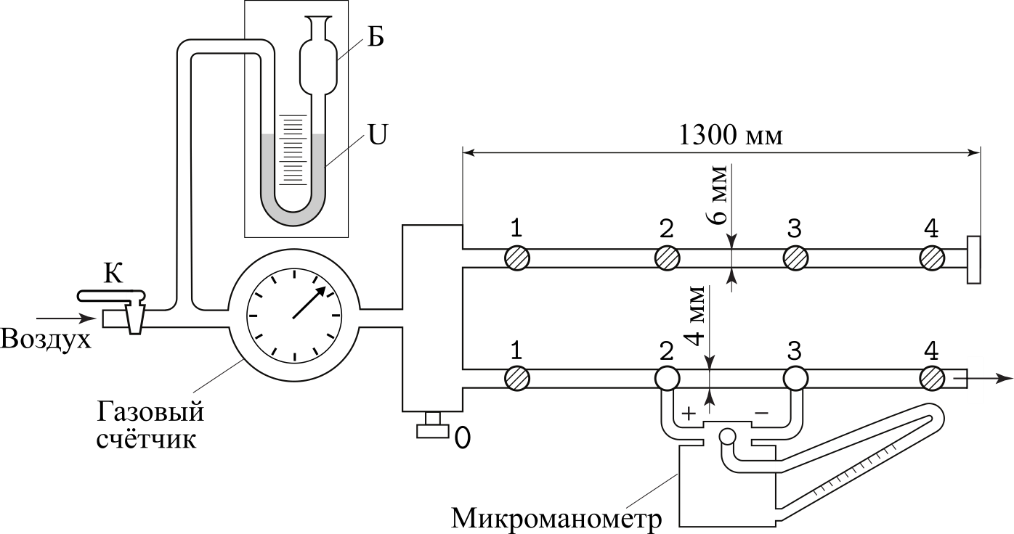
\includegraphics[width=0.7\linewidth]{setup.png}
\label{fig:setup}
\caption{Экспериментальная установка}
\end{figure}

\paragraph{}
Через кран К в экспериментальную установку попадает газ под давлением чуть более высоким, чем атмосферное.
За краном К установлен U-образный манометр показывающий разницу в давлении между входящим воздухом и атмосферой. 
Если давление в установке поднимается выше допустимого вода в манометре поднимается в баллон Б, который издаёт звук оповещающий экспериментатора.
Далее воздух проходим через газовый счётчик, измеряющий объём прошедшего через него газа.
После этого газ проходит через одну из двух трубок с заглушками, к которым можно подключать концы микроманометра.


\subsection{Ход эксперимента}

\begin{enumerate}
\renewcommand{\labelenumi}{\textbf{\Roman{enumi}.}}
\renewcommand{\labelenumii}{\arabic{enumii}.}

\item Подготовим установку к работе:
	\begin{enumerate}
	\item
	Ознакомимся  с  устройством  и  характеристиками  приборов  (газового счётчика и 			спиртового микроманометра); Проверим их   предварительную настройку и регулировку 			согласно техническому описанию установки;
	\item 
	Ознакомимся с измерительными шкалами приборов, запишем рабочий диапазон и цену деления; предварительно оценим инструментальные погрешности (по паспортам приборов и/или по цене деления их шкал).
	\end{enumerate}
	
\item Проведём предварительный запуск установки и убедимся в её работоспособности:
	\begin{enumerate}
	\item Подсоединим манометр к двум соседним выводам на конце одной из трубок 				(рекомендуется начать с трубки диаметром $d \approx 4$ мм). Убедимся, что все отверстия, кроме одного -- выходного -- плотно завинчены пробками.
	\item Убедимся, что кран К, соединяющий компрессор с установкой, закрыт. Включим компрессор. Переведите рычажок микроманометра в рабочее положение (+).
	\item Медленно приоткрывая кран К и непрерывно контролируя показания микроманометра, создадим небольшой поток воздуха через трубку. 
	\item Пронаблюдаем за показаниями приборов в зависимости от интенсивности потока  через  трубку.  Убедимся в том,  что  при  неизменном  положении крана К показания манометра стабильны, а стрелка расходомера вращается равномерно.
	\end{enumerate}
	
\item Измерим параметры окружающей среды: \textbf{температуру}, \textbf{влажность воздуха} и \textbf{атмосферное давление}. В ходе дальнейшей работы проследим за этими показаниями и при необходимости зафиксируем их изменения. Запишем \textbf{диаметры трубок} (указаны на установке). Зарисуем схему расположения  измерительных отверстий  на трубках с  указанием  расстояний между ними.

\item Проведите предварительные расчёты:
	\begin{enumerate}
	\item Рассчитаем значение расхода $Q_{\text{кр}}$, при котором число Рейнольдса в трубке станет равным критическому $Re_{\text{кр}} \approx 10^3$. Для предварительной оценки прими вязкость воздуха равной $\eta_\text{возд} \approx 2 \cdot 10^{-5}$ Па $\cdot$ с, плотность воздуха определим по уравнению идеального газа. В качестве характерной скорости  потока используем её  среднее  значение $\bar{u} = Q/ \pi R^2$.
	\item По формуле Пуазейля *7* рассчитайте соответствующий перепад давления выбранном вами участке $\Delta P_\text{кр}$. Выразим значение $\Delta P_\text{кр}$ в делениях шкалы микроманометра.
	\item По формуле *8* оценим длину $l_\text{уст}$, на которой течение можно считать установившимся при $Re \approx Re_\text{уст}$. Проверим, можно ли считать устано-вившимся течение на участке, выбранном для проведения измерений.
	\end{enumerate}
	
\item Меняя расход воздуха краном К и наблюдая за столбиком спирта в микроманометре, визуально определим границу перехода $\Delta P_\text{кр}$ ламинарного течения  к  турбулентному  (турбулентный  режим  характеризуется заметными пульсациями давления во времени).Сравним полученное экспериментально $\Delta P_\text{кр}$ оценкой, проведенной в п. 4.

\item Подберём параметры измерения расхода газа $Q = \Delta V / \delta t$, так	чтобы его относительная погрешность составила не более $\varepsilon = 1\%$.
	\begin{enumerate}
	\item
	\end{enumerate}

\end{enumerate}

\FloatBarrier

\subsection{Обработка экспериментальных данных}

\medskip\hrule\medskip

\section{Выводы}

\medskip\hrule\medskip

\end{document}
